\begin{figure}[!t]
\centering
\vspace{-0.2in}
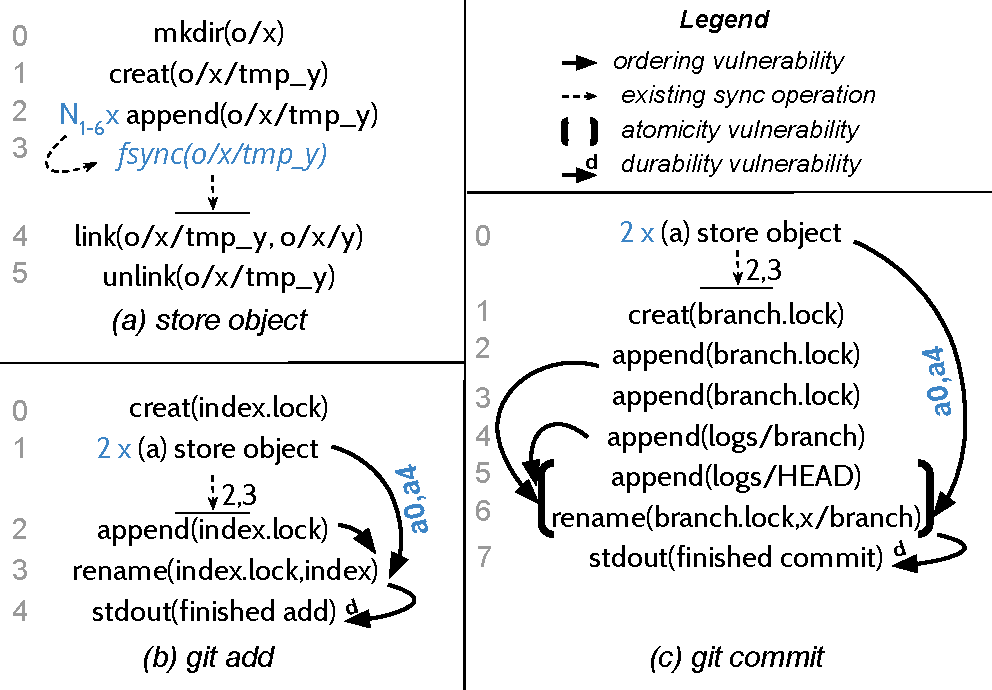
\includegraphics[scale=0.47]{figs/git2.pdf}
\vspace{-0.1in}
\mycaption{fig-git}{Git Update Protocol}{\footnotesize The figure shows the
update protocol of Git broken up into modules. The dark arrows and brackets represent
new dependencies discovered by \toolname. The dashed arrows represent
known dependencies. Numbers on the arrow represent the lines of
the source module that need to be persisted before the destination. We observe that
even though Git is a mature, well-tested application, crash vulnerabilities
exist in common tasks such as add and commit.
}
\vspace{-0.2in}
\end{figure}


